% Chapter Template
\part{Physics introduction}
\chapter{The Standard Model and Beyond} \label{Chapter1} 

\section{Introduction}
Starting from the late 19th century and progressing in the first half of the 20th century, 
the theories and discoveries of thousands of physicists have led to a significant insight into the fundamental structure of matter. 
By the 1960s, physicists had proposed quite a collection of what they assumed to be fundamental particles, basic building blocks of matter that could not be resolved any further into sub-pieces. 

In 1964, theorists Murray Gell-Mann~\cite{GELLMANN1964214} and George Zweig~\cite{Zweig:570209} theorized that many components of the so-called ``particle zoo'' were composite particles which consists of even smaller parts, which are now called quarks. Thus the list of fundamental particles was further reduced and the description of the fundamental forces which govern the interaction between particles themselves was added. This was the outset of the development of the Standard Model of particle physics.
The first references to the so-called “standard model” can be found in papers published in the 1970s~\cite{Pais:1975gn,PhysRevD.13.680} and only in the '80s and '90s the \emph{S} and \emph{M} got capitalized.

To this day, the Standard Model (SM) has successfully interpreted nearly all experimental results and accurately predicted a wide variety of phenomena, getting even more credit with the latest discoveries such as top quark observation (1995)~\cite{Abachi_1995} and Higgs boson discovery (2012)~\cite{20121,201230}.\\
Even though it is considered the most solid description of the subatomic world, it falls short when trying to address the full picture. Those unexplained physics observations have inspired the big hunt for new physics that has drawn the creation of so many new experiments and that has fed fresh exotic theories. \\
This thesis cooperates in this attempt by confronting one of those exotic models with the experimental data. 


\section{The Standard Model of Elementary Particles}\label{sec:sm}
Figure~\ref{fig:SMfig} shows the building blocks of the Standard Model. They are either matter particles, everyday matter
or exotic matter created in particle accelerators and in the early universe, or they are the additional force-carrier particles.

In the SM, the elementary particles are grouped into two main categories on the basis of the statistic they obey and consequently of the spin: fermions and bosons. 
\begin{figure}[h]
\centering
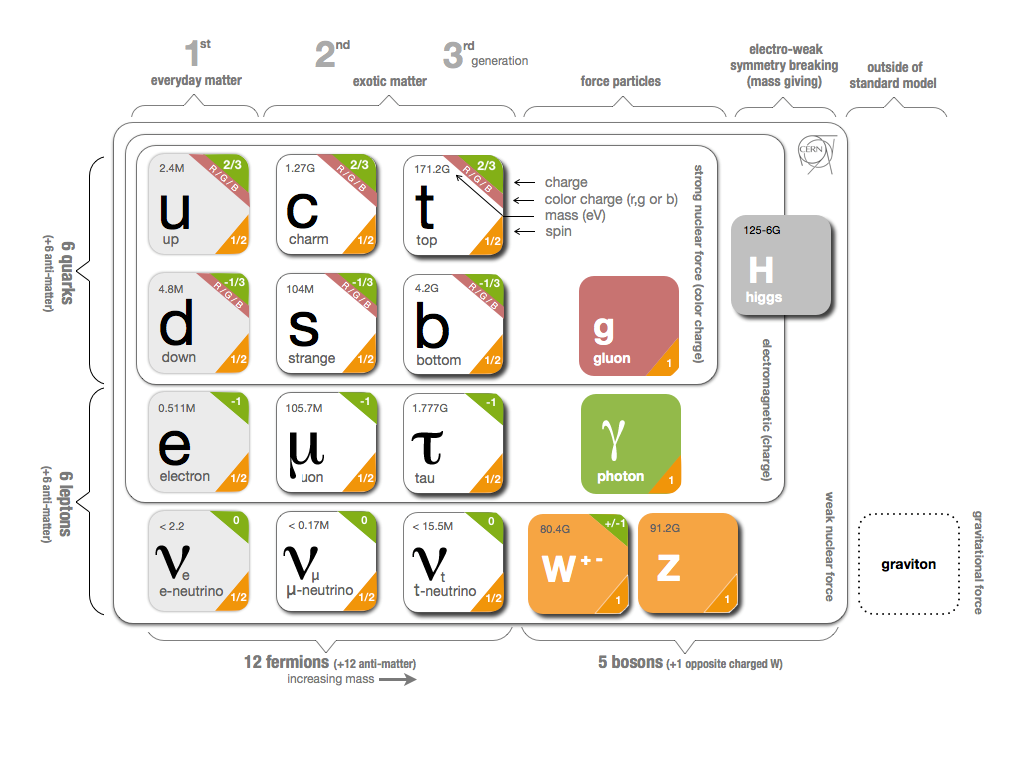
\includegraphics[clip,trim=1cm 2cm 2cm 1cm, width=0.75\textwidth]{Figures/c1/SMinfographic_image.png}
\caption{Elementary particles of the Standard Model (infographic
  developed for~\cite{particlefest})}
\label{fig:SMfig}
\end{figure}

The fermions are particles which follow Fermi-Dirac statistics and correspondingly have half odd integer spin (1/2, 3/2, 5/2...). They obey the Pauli exclusion principle and therefore they have different symmetry properties, as opposed to bosons, when exchanging of two identical particles: the total wave function of a system of two identical fermions is antisymmetric for fermions. This leads to the fact that, in a rigorous way, if two identical (in spin and space coordinates) fermions interchange, the total wave function changes its sign. Thus, two or more identical fermions can not simultaneously exist in the same quantum state. On the contrary particles with an integer spin like the bosons which follow Bose-Einstein statistics do not obey the Pauli exclusion principle and can occupy the same quantum state. 


In the Standard Model, there are two types of elementary fermions: quarks (which form hadrons such as protons and neutrons) and leptons. 
Moreover, the fermions are grouped into three generations and each generation has two types of leptons and two quarks. One of the two leptons have one electric charge -1, the other one is neutral; the two quarks have charges $-1/3$ (down-type) and $+2/3$ (up-type). Between generations electric and strong interactions are identical while particles differ by their flavor quantum number and mass.  The first generation consists of electrons ($e$) and electron neutrinos ($\nu_e$) and of \emph{up} and \emph{down} quarks. All the everyday matter is composed by up-down quarks and electrons. The second generation is made of muons ($\mu$) and muon neutrinos ($\nu_\mu$) and of \emph{charm} and \emph{strange} quarks. The third generation is composed by taus ($\tau$) and tau neutrino ($\nu_\tau$) and by \emph{top} and \emph{bottom} quarks. The particles of higher generations have larger masses than the preceding ones, this has the effect that leptons and quarks of the second and third families are more unstable with shorter life-times and can easily decay back to elements from the first generation.\\
Each of the 12 fermions has an anti-matter particle which presents all the charges with opposite sign.

The fermions interact by exchanging bosons. The elementary bosons are force carriers and each of them is associated with a fundamental force. The photon ($\gamma$) is the mediator of the electromagnetic force, it has spin equal to 1, it is neutral and massless. The $\PW^{\pm}$ and \PZ are mediators of the weak force, they have spin 1, the $\PW^{\pm}$ have unitary charge (+1 or -1) while \PZ is neutral; the are heavy in mass ($M_\PW =\:$80.379 $\pm$ 0.012\GeV~\cite{pdgw}, $M_\PZ =\:$91.1876 $\pm$ 0.0021\GeV~\cite{pdgz}) and very short-lived. The quarks possess color charge which means they are subject to the strong interaction mediated by the gluons ($g$) which likewise are associated to a color charge. Because of a property of the strong interaction known as \emph{color confinement}, quarks can not exist isolated. Therefore quarks and gluons must cluster together to form hadrons which are color neutral (white) and which can exist and propagate freely. The hadrons can be made of either a quark and an anti-quark, \emph{mesons} or three quarks, \emph{baryons}. The mesons are composite bosons (spin 0 or 1) while baryons are composite fermions. Quarks, besides interacting through strong force, can also transform into quarks of another flavor through the weak interaction by absorbing/emitting a \PW boson. The strengths/probabilities of the weak interactions between the six quarks do not have all the same magnitude (some are more preferable) and they are described by the values in the Cabibbo–Kobayashi–Maskawa matrix~\cite{10.1143/PTP.28.870}.\\
The massive bosons get their mass thanks to the interaction with the quantum field of the Higgs boson. The so-called Brout–Englert–Higgs (BEH) mechanism refers to the generation of masses for the three weak gauge bosons (\PW, \PZ) through electroweak symmetry breaking~\cite{PhysRevLett.13.321,PhysRevLett.13.508}. The mathematical treatment of the Standard Model and of the BEH mechanism is presented in Sec.\ref{sec:mathSM}.\\
The last fundamental force, gravity, is not included in the Standard Model framework. 

The leptons are not affected by the strong interaction while they are subject to electromagnetic and weak interactions. As already said, the six leptons are organized in three generations, then are arranged in three left-handed weak isospin doublets where charged and neutral leptons share the same left-handed helicity. Each doublet has a different lepton number which has to be conserved during all the interactions implying that leptons and anti-leptons must be created in pairs of a single generation. The only violation of this universal lepton number conservation can be observed in the weak interaction in the neutrino oscillations where transformations between different generations occur. The neutrino oscillation and the obvious consequences are going to be extensively explained in Sec.~\ref{sec:bsm}. 


\section{The mathematical formulation of the Standard Model}\label{sec:mathSM}
This section describes the mathematical framework of the Standard Model of particle physics, which is a gauge Quantum Field Theory (\emph{QFT}). For an extensive discussion and explanation of QFT and of the Standard Model refer to~\cite{Bardin:1999ak}.
\subsection{Quantum Field Theory and Gauge invariance}\label{sec:qft}
In a QFT theory, the fundamental objects are described as quantum fields with specific transformation properties governed by a set of symmetry groups. The fields are: the \emph{fermion} fields $\psi$, the \emph{electroweak boson} fields $W_1, \; W_2, \; W_3,$ and $B$, the \emph{gluon} field $G_a$ and the Higgs field $\phi$. The dynamics of those quantum fields are completely determined by the Lagrangian density, $\mathcal{L}$. \\
The description of QFT starts with a Lagrangian density $\mathcal{L}$, a function of the fields in the system and their derivatives, and possibly the space-time coordinates; minimizing the action ($\mathcal{S}$), which is the space-time integral of $\mathcal{L}$, the equation of motion can be extracted:
\begin{equation}
\label{eq:action}
 \mathcal{S} \;\; = \;\; \int \mathcal{L}(x) \ d^4x,
\end{equation}
where x is the space-time coordinate.

The complete Standard Model Lagrangian contains specific terms for every one of the fundamental interactions. In the rest of the section all these elements and the corresponding meanings are going to be illustrated and clarified.

To start, consider the Lagrangian of a free spinor field $\psi$ which contains a kinetic and mass term:
\begin{equation}
\label{eq:dirac}
 \mathcal{L}_{Dirac} \;\; = \;\; \overline{\psi}(x)\ (i\gamma^{\mu}\partial_{\mu} - m ) \psi(x)
\end{equation}
where the Einstein notation is used which implies summation over the indices $\mu \in 0,1,2,3$; $m$ is the fermion's mass, $\gamma^{\mu}$ are the gamma matrices ($\gamma^{\mu}\gamma^{\nu} + \gamma^{\nu}\gamma^{\mu} = 2g^{\mu\nu}$ with $g^{\mu\nu}$ is the Minkowski metric) and $\partial_{\mu}$ is the space-time derivative $(\nicefrac{\partial}{\partial_{t}}, \nicefrac{\partial}{\partial_{x}}, \nicefrac{\partial}{\partial_{y}}, \nicefrac{\partial}{\partial_{z}})$. The $\psi(x)$ denotes the Dirac fermion field and the anti-fermion field, the adjoint spinor $\overline{\psi}(x)$ is defined as $\psi^\dag\gamma^{0}$, with $\psi^\dag$ the hermitian conjugate of $\psi$.

The Standard model is a gauge quantum field theory which means it is based on the hypothesis that some symmetries, \ie transformations that leave the Lagrangian of the system unchanged, are possible not only globally, but also locally.
Most theories of physics are described by Lagrangians who are invariant under certain transformations of the coordinate system performed simultaneously at every point in spacetime: they are therefore said to have global symmetries. A local symmetry is one that keeps a property invariant when a possibly different symmetry transformation is applied at each point of spacetime; specifically a local symmetry transformation is parameterized by the spacetime co-ordinates, whereas a global symmetry is not. The concept underlying gauge theories is precisely the postulate that Lagrangians must also possess local symmetries, i.e. gauge symmetries and gauge invariant.\\
Going back to Eq.~\ref{eq:dirac}, this Lagrangian is invariant under a global U(1) phase transformation
\begin{equation}
\label{eq:globalT}
 \psi(x) \rightarrow \psi'(x) = e^{-i\omega} \psi(x), \; \; \; \; \; \;    \overline{\psi}(x) \rightarrow \overline{\psi'}(x) = e^{i\omega} \overline{\psi}(x),
\end{equation}
where $\omega$ is a constant. Thus, the requirement is for this Lagrangian to be invariant under a local U(1) transformation
\begin{equation}
\label{eq:localT}
 \psi(x) \rightarrow \psi'(x) = e^{-i\omega(x)} \psi(x), \; \; \; \; \; \;    \overline{\psi}(x) \rightarrow \overline{\psi'}(x) = e^{i\omega(x)} \overline{\psi}(x),
\end{equation}
where now $\omega(x)$ is a function of the spacetime point $x$. Considering then that $\partial_{\mu}$ would also act on $\omega(x)$, to make the 
Lagrangian invariant under this gauge symmetry, a new term, vector field, $A_{\mu}$ has to be introduced in Eq.~\ref{eq:dirac}:
\begin{equation}
\label{eq:GS1}
 \mathcal{L}_{Dirac} \;\; = \;\; \overline{\psi} (i\gamma^{\mu} (\partial_{\mu} + igA_{\mu})-m) \psi \;\;\; \equiv  \;\;\; \overline{\psi} (i\gamma^{\mu}\mathcal{D}_{\mu}-m) \psi 
\end{equation}
(the $(x)$ dependence is omitted from the notation).\\
 $A_{\mu}$ is the gauge field which couples to the spinor field $\psi$ with a coupling strength $g$; $\mathcal{D}_{\mu}$ is called covariant derivate and it is defined as $\mathcal{D}_{\mu} = \partial_{\mu} + igA_{\mu}$. \\
The $\mathcal{L}_{Dirac}$ in Eq.~\ref{eq:GS1} is invariant under local trasformation ($\mathcal{L}_{\psi} =\mathcal{L}_{\psi'}$) requiring:
\begin{equation}
\label{eq:GS2}
A_{\mu} \rightarrow A'_{\mu} =  A_{\mu} + \frac{1}{g}[\partial_{\mu} \omega(x)]
\end{equation}

This example has made it clear that asking the Lagrangian to be gauge invariant under a certain gauge transformation, gauge fields are naturally introduced in the $\mathcal{L}$ itself. These fields entail the existence of the gauge bosons, spin 1 particles, which couple to the fermions. \\
Defining the field strength tensor $F_{\mu\nu} = \partial_{\mu}A_{\nu} - \partial_{\nu}A_{\mu}$\footnote{The field strength tensor is defined as $F^{a}_{\mu\nu} = \partial_{\mu}A^{a}_{\nu} - \partial_{\nu}A^{a}_{\mu} + g f^{abc} A^{b}_{\mu}A^{c}_{\nu}$ for the gauge field $A_{\mu}$ with gauge constant $g$. The structure constant $ f^{abc}$ vanish since U(1), here used, in an Abelian commutative group.}
, the final gauge invariant $\mathcal{L}_{Dirac}$ can be written as
\begin{equation}
\label{eq:GS3}
 \mathcal{L}_{Dirac} \;\; = \;\; -\frac{1}{4} F_{\mu\nu} F^{\mu\nu} + \overline{\psi} (i\gamma^{\mu} (\partial_{\mu} + igA_{\mu})-m) \psi \;\;\;\;\;\; \footnote{In this equation the mass term is not invariant under local transformations. The boson remain massless up to this point, the concept of spontaneous symmetry breaking is going to be introduced later in Sec~\ref{sec:symBreaking}}
\end{equation}

\vspace{10mm}
The example here was carried out for a U(1) unitary transformation which can be described by one ($n^2$) degree of freedom (or generator of the gauge group U(1)). U(1) is an Abelian commutative group.  \\
As preface for the next section the general case for a special unitary group of order \emph{n}, SU(\emph{n}), is presented here. The special unitary group SU(\emph{n}) is the Lie group of  $n\times n$ matrices with determinant 1. The group is described by a set of $n^2 -1$ gauge generators, $T^a$ with $a \in (1, 2, ... , n^2 -1)$. The covariant derivate of SU(\emph{n}) is then $\mathcal{D}_{\mu} = \partial_{\mu} + igT^aA^a_{\mu}$ and it corresponds to an $n\times n$ matrix. At the same time, there are $n^2 -1$ gauge bosons which construct the currents and mediate the interaction.\\
The gauge group can be Abelian, like U(1), or non-Abelian; the latter case means that the generators of the group do not commute. At a different level, it means the field strength tensor and the kinetic term for the gauge fields in the Lagrangian naturally allows for
self–interactions of the gauge bosons. A theory with a local non-Abelian phase transformation is called a Yang-Mills theory.


\subsection{The Standard Model gauge group}\label{sec:gauge group}
Three symmetries are identified to be necessary and sufficient in the SM theory to address and describe the experimental results of the particles and of their interactions. The Standard Model is described by a $SU(3)$ $\otimes$ $SU(2)$ $\otimes$ $U(1)$ gauge symmetry group; each subgroup has the corresponding gauge fields.\\
As it was explained in the previous section, the SM Lagrangian manifests a $U(1)$ local phase invariance. The associated gauge field to this Abelian invariance of the theory is called $B_\mu$. There is then the second invariance, under non-Abelian transformations that build an $SU(2)$ group, which introduces three $W^i_\mu$ fields ($i = 1,2,3$), one for each of the three generators of $SU(2)$. The last invariance non-Abelian that forms $SU(3)$ leads to the introduction of eight $G^a_\mu$ fields ($a = 1,...,8$).\\
The covariant derivative which guarantees the full SM Lagrangian to be invariant under the three transformation described above is:
\begin{equation}
\label{eq:SMderivative}
\mathcal{D}_{\mu} \;\; = \;\; \partial_{\mu} + ig_1\frac{Y}{2}B_{\mu} - ig_2\frac{\sigma^i}{2}W^i_{\mu} - ig_s\frac{\lambda^a}{2}G^as_{\mu}
\end{equation}
where $Y$, $\sigma^i$ and $\lambda^a$ represent the generators for the $U(1)$ weak hypercharge, the $SU(2)$ weak isospin and the $SU(3)$ color space, respectively. The $SU(2)$ generators in the third term of Eq.~\ref{eq:SMderivative} are the $2\times2$ Pauli-matrices $\sigma^i$ and the $SU(3)$ generators, the forth term in~\ref{eq:SMderivative}, are the $3\times3$ Gell-Man matrices $\lambda^a$ ($a = 1,...,8$).\\

In the following sections the distinct terms in the full SM Lagrange are introduced and explained. Starting from the $\mathcal{L}_{Dirac}$ in Eq.~\ref{eq:GS1} and using the covariant derivative of Eq.~\ref{eq:SMderivative}, the SM Lagrangian becomes then invariant under the three gauge groups transformations. Thus, it is described the fermion behaviors under the gauge transformations and their interactions among all the particles of the SM. 

\subsubsection{The Electroweak theory}\label{sec:ewk}
The Electroweak theory gives a unified description of the electromagnetic and the weak forces, by asking gauge invariance under the $SU(2)_{L}$ $\otimes$ $U(1)_{Y}$ gauge symmetry group, with the subscript $L$ referring to the left-handed chiral structure of $SU(2)$.\\
Introducing the chiral projection operators:
\begin{equation}
\label{eq:LRoperators}
P_L=\frac{1}{2} (1-\gamma^5), \;\;\;\ P_R=\frac{1}{2} (1+\gamma^5), \;\; \;\; \;\; (\text{defining} \;\; \gamma^5 = i\gamma^0\gamma^1\gamma^2\gamma^3)
\end{equation}
the Dirac spinors $\psi$ can be projected onto the right-handed (RH) chiral states and the left-handed (LH) chiral states as:
\begin{equation}
\label{eq:LR1}
\psi = \begin{pmatrix}
\psi_L\\
\psi_R
\end{pmatrix}
\end{equation}
with $\psi_L$, $\psi_R$ as left- and right-handed Weyl spinors. Replacing the spinor in the Lagrangian, massless fermions are decoupled into LH and RH particles:
\begin{equation}
\label{eq:LR2}
\overline{\psi} \gamma^{\mu} \psi \;\; = \;\; \overline{\psi}_L\gamma^{\mu} \psi_L +  \overline{\psi}_R\gamma^{\mu} \psi_R
\end{equation}
where, for massless fermions, their chirality coincides with their helicity. Sustained by clear experimental results for the parity-violating nature of the ElectroWeak theory, the weak-isospin charge appears to be different for particles with different chirality and it looks that the corresponding gauge fields interact only with LH fields. Thus the LH fermions fields are grouped in doublets, for example ($e_L,\nu_{eL}$) or ($u_L,d_L$), while the RH fermions transform as singlets with zero isospin and as consequence do not interact with the gauge bosons of $SU(2)$. When the RH massless fermions do not couple with any of the interactions, they are called \emph{sterile} and they are not part of the SM theory.\\
Another important consequence of the chiral nature of the isospin transformations is that the mass term can be written as:
\begin{equation}
\label{eq:LR3}
m\overline{\psi} \psi \;\; = \;\; m(\overline{\psi}_R\psi_L +  \overline{\psi}_L\psi_R)
\end{equation}
which violates the $SU(2)$ gauge invariance. 

The physical gauge fields of the EW  theory are the neutral \PZ boson field $\PZ^0_{\mu}$, the two charged \PW boson fields $\PW^{\pm}_{\mu}$ and the photon field $A_{\mu}$. Those physically observable gauge fields are the linear superposition of the gauge fields of the $SU(2)_{L}$ $\otimes$ $U(1)_{Y}$ gauge group according to:
\begin{align}
Z^0_{\mu} \; &= \; \cos\theta_{W} W^3_{\mu} - \sin\theta_{W} B_{\mu} \label{eq:z}\\
W^{\pm}_{\mu} \; &= \; \sqrt{\frac{1}{2}}(W^1_{\mu} \mp iW^2_{\mu}) \label{eq:w}\\
A_{\mu} \; &= \; \sin\theta_{W} W^3_{\mu} + \cos\theta_{W} B_{\mu} \label{eq:photon}
\end{align}
where the $\theta_W$ is the Weinberg angle defined as:
\begin{equation}
\label{eq:weinberg}
\tan \theta_W = \frac{g_1}{g_2}
\end{equation}

The relevant quantum numbers related to the $SU(2)_{L}$ $\otimes$ $U(1)_{Y}$ gauge group transformations are the weak isospin, $T$ in particular the third component of it, $T_3$ and the weak hypercharge $Y$. As a convention, the quantum number for left-handed leptons is chosen to be $Y = -1$. All the quantum numbers of the RH and LH fermions can be derived using the following relations: $Y_R = 2Y_L$ and $Y = 2(Q_{EW}-T_3)$.\\

To summarize, a theory of massless fermions and EW bosons was described. The theory defines electromagnetic interactions between the photon field and the charged fermions; it includes charged and neutral current interactions between the fermions and the \PW and \PZ bosons respectively and finally allows self–interactions between the gauge bosons. 

\subsubsection{QCD, Quantum Chromodynamics}
The description of the strong nuclear force in the SM is introduced by the theory of Quantum Chromodynamics which defines the interaction between quarks and gluons.\\
The SM Lagrangian is invariant under $SU(3)_C$ gauge transformations; as previously described, $SU(3)_C$ is a non-abelian group, with eight generators, the $3\times3$ Gell-Man matrices $\lambda^a$ ($a = 1,...,8$) and eight massless gauge bosons fields $G^a_{\mu}$ called gluons. The subscript ``$C$'' refers to the color quantum number or color charge, therefore the strong interaction only interests color particles, quark and gluons , while the other fermions and boson are singlets under this gauge symmetry. \\ 
The strong coupling constant ($g_s$ in Eq.~\ref{eq:SMderivative}) decreases as the energy of the interaction that is probed increases; this phenomenon is called as asymptotic freedom and leads to the principle of color confinement as explained in the previous section~\ref{sec:sm}. This means that the quarks can neither exist nor be observed as individual asymptotic states, thus they are always clustered in at least a pair or multi-quark particles called hadrons.


\subsubsection{Electroweak symmetry breaking}\label{sec:symBreaking}
As anticipated in section~\ref{sec:ewk}, the theory still encloses no mass term for the fermions (Eq.~\ref{eq:LR3}) since it would not be invariant under gauge transformations. The same issue appears for the mass term $-m^2A_{\mu}A^{\mu}$ in the bosons gauge fields of Eq.~\ref{eq:z}-~\ref{eq:w}. Up to this point the fermions and bosons are massless.

The mechanism proposed to explain the particle masses and generate in a gauge invariant way is referred to as spontaneous symmetry breaking.\\
In the SM this mechanism is called the Brout-Englert-Higgs (BEH) mechanism, proposed by Robert Brout, Francois Englert and Peter Higgs in 1964~\cite{PhysRevLett.13.321,PhysRevLett.13.508}. It introduces a complex scalar field $\phi$, defined as a doublet in $SU(2)_{L}$ space and with non-zero hypercharge under $U(1)_Y$ and represented as a singlet in $SU(3)_{C}$ color space:
\begin{equation}
\label{eq:higgsphi}
\phi = \begin{pmatrix}
\phi^+\\
\phi^0
\end{pmatrix}
\end{equation}
with $\phi^+$ and $\phi^0$ complex fields. The Higgs field Lagrangian is:
\begin{equation}
\label{eq:higgsL}
 \mathcal{L}_{H} \;\; = \;\; (D^{\mu}\phi)^\dag (D_{\mu}\phi) - V(\phi) \;\; = \;\; (D^{\mu}\phi)^\dag (D_{\mu}\phi) - \mu^2\phi^\dag \phi - \lambda(\phi^\dag \phi)^2
\end{equation}
where $V(\phi)$ is the scalar potential, $\mu^2$ is a mass parameter, $\lambda > 0$ is a dimensionless parameter which quantifies the self-interaction strength of the Higgs field. When $\mu^2 > 0$ the potential $V(\phi)$ has a global minimum for $\phi = 0$, while when $\mu^2 < 0$ the potential, takes the shape of a so called ``Mexican hat potential'', and has non-zero degenerate minima at:
\begin{equation}
\label{eq:higgsM}
\phi^\dag \phi \;\; = \;\; - \frac{\mu^2}{2\lambda} \;\; \equiv \;\; \frac{v^2}{2}
\end{equation}
with $v$ is the vacuum expectation value (VEV) of the Higgs field. A simplified representation of the two cases can be visualized in Figure.~\ref{fig:mexico}.

\begin{figure}[h]
\centering
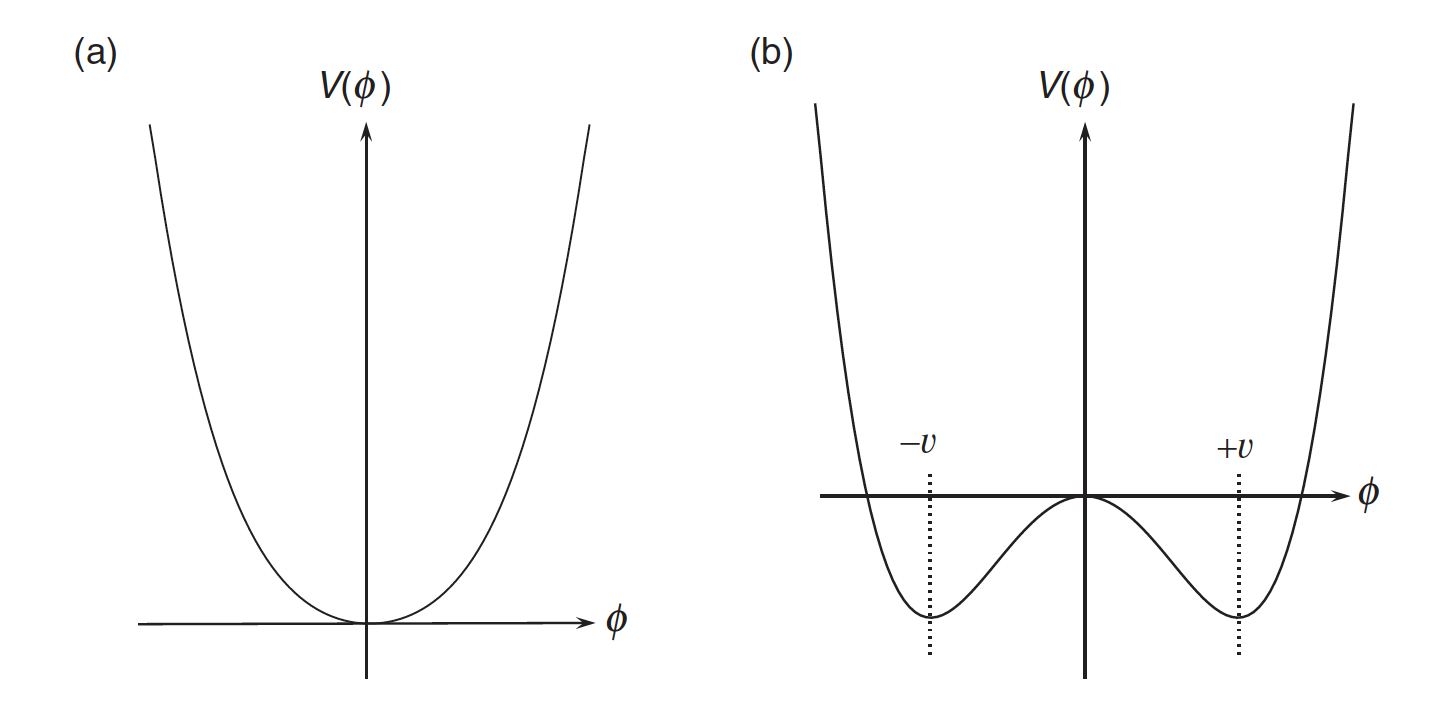
\includegraphics[width=0.55\textwidth]{Figures/c1/higgsPotential}
\caption{One dimensional representation~\cite{thomson_2013} of the Higgs potential in case (a) of $\mu^2 > 0$ and minimum for $\phi = 0$ for an unbroken theory and in case (b) for $\mu^2 < 0$ and VEV for a spontaneous symmetry breaking.}
\label{fig:mexico}
\end{figure}

Starting from Eq.~\ref{eq:higgsM}, it can be written $\phi^+=\nicefrac{(\phi_1 + i\phi_2)}{\sqrt{2}}$ and $\phi^0=\nicefrac{(\phi_3 + i\phi_4)}{\sqrt{2}}$ and knowing $2\phi^\dag \phi = \phi^2_1+\phi^2_2+ \phi^2_3+ \phi^2_4 = v^2$ it is clear that the minima form a four-dimensional sphere.\\
Furthermore, studying the region of the vacuum and choosing a particular vacuum in the $SU(2)$ space with $\phi_3 = v$ and $\phi_1=\phi_2=\phi_4=0$, it is possible to expand around the minimum and write:
\begin{equation}
\label{eq:higgsphi2}
\phi(x) = \frac{1}{\sqrt{2}}\begin{pmatrix}
0\\
v+ h^0
\end{pmatrix}
\end{equation}
where $h^0$ is a scalar Higgs field. Now combining and replacing~\ref{eq:SMderivative} and~\ref{eq:higgsphi2} into the Lagrangian~\ref{eq:higgsL} it happens that photon field remains massless while the two mass terms for \PW and \PZ bosons are naturally obtained:
\begin{align}
m^2_W &= \frac{g_2^2v^2}{4}\label{eq:massW}\\
m^2_Z &= \frac{(g_1^2+g_2^2)v^2}{4}\label{eq:massZ}
\end{align}
Identifying those terms with the electroweak gauge-bosons allows for the extrapolation of the expectation value $v = \sqrt{\nicefrac{\mu^2}{\lambda}} = 246$\GeV of the Higgs field in the vacuum.
The three components $\phi_1,\phi_2$ and $\phi_4$ are referred to as massless Goldstone bosons and, as it was shown before, in a specific gauge choice called \emph{unitary gauge} ($\phi_3 = v$ and $\phi_1=\phi_2=\phi_4=0$) they do vanish. The remaining degree of freedom, the scalar field $h^0$, is known as Brout-Englert-Higgs boson. The mass of this SM Higgs boson is equal to $\sqrt{2\lambda}v$, with $\lambda$ being a free parameter in the SM, and
hence, there is no a priori prediction for the Higgs mass. The experimental measurements of the Higgs boson mass state  $m_{h^0}=125.10\pm0.14$\GeV~\cite{pdgw}. 

\begin{figure}[h!]
\centering
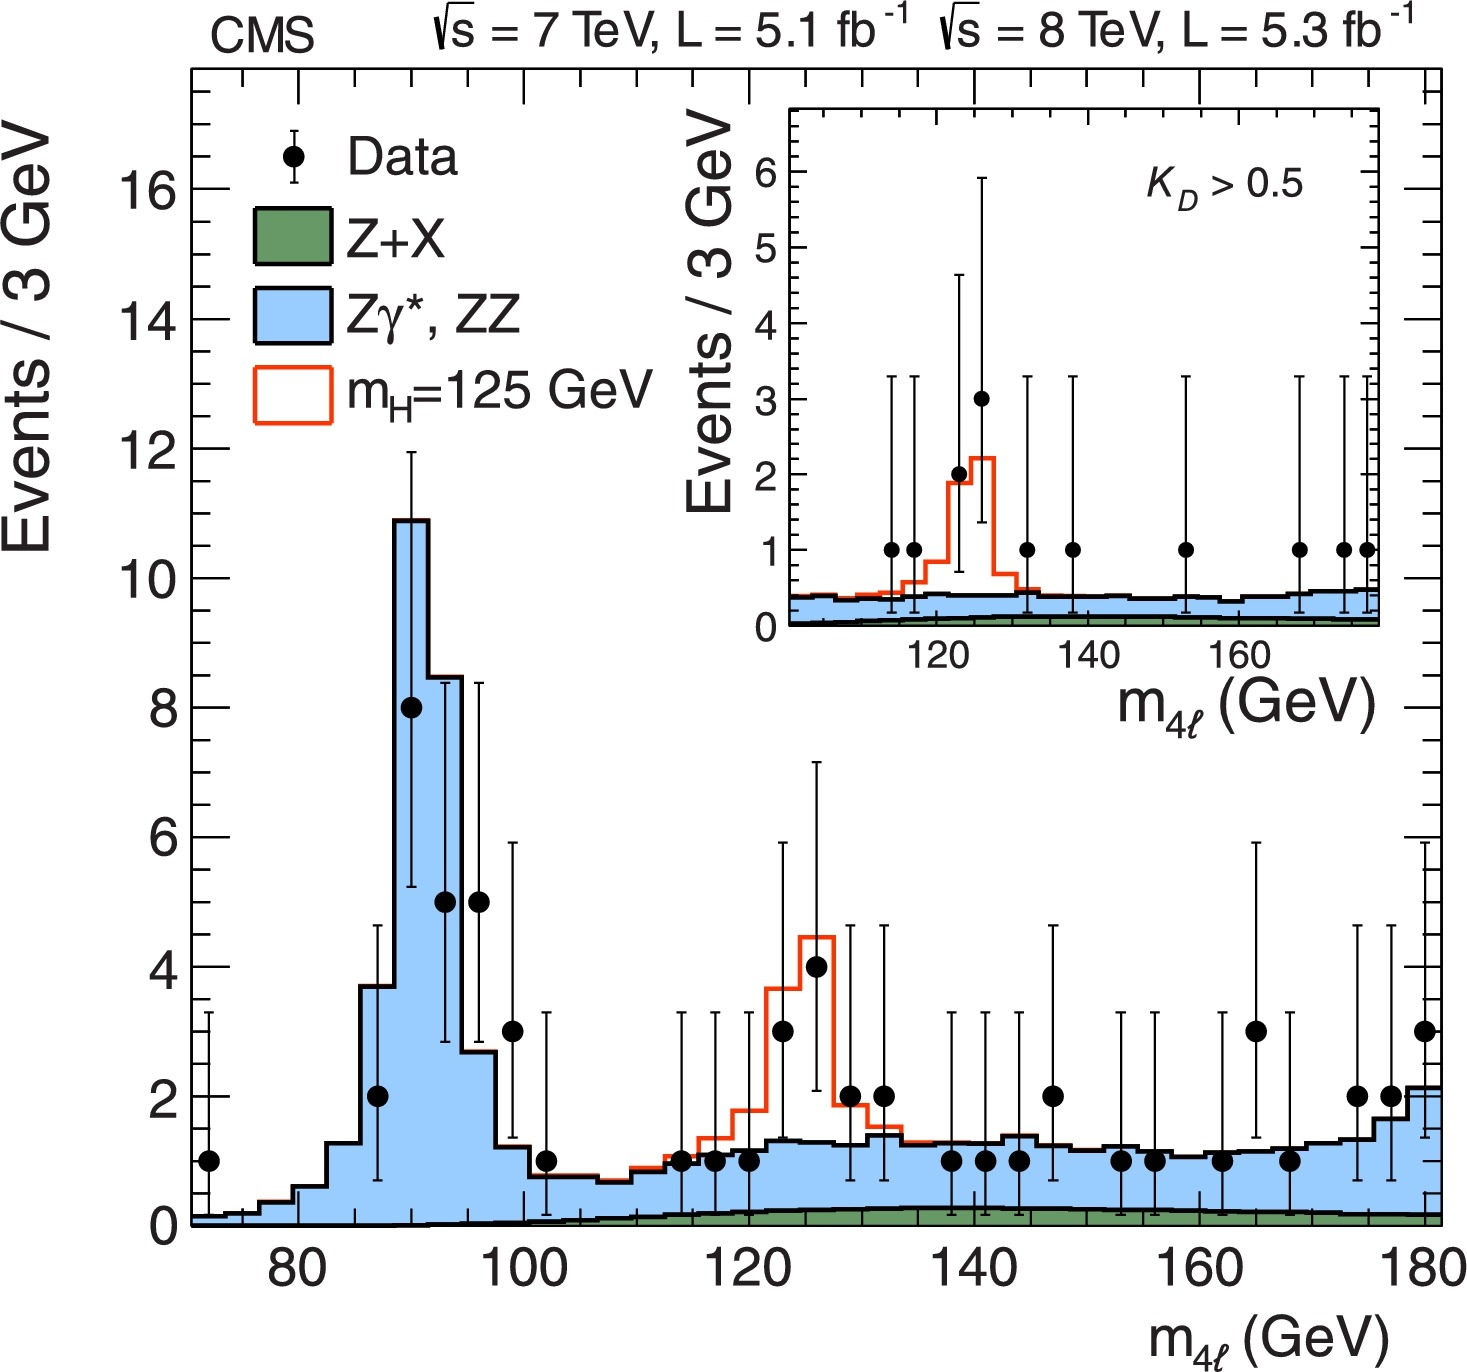
\includegraphics[width=0.45\textwidth]{Figures/c1/higgs_1.jpeg}
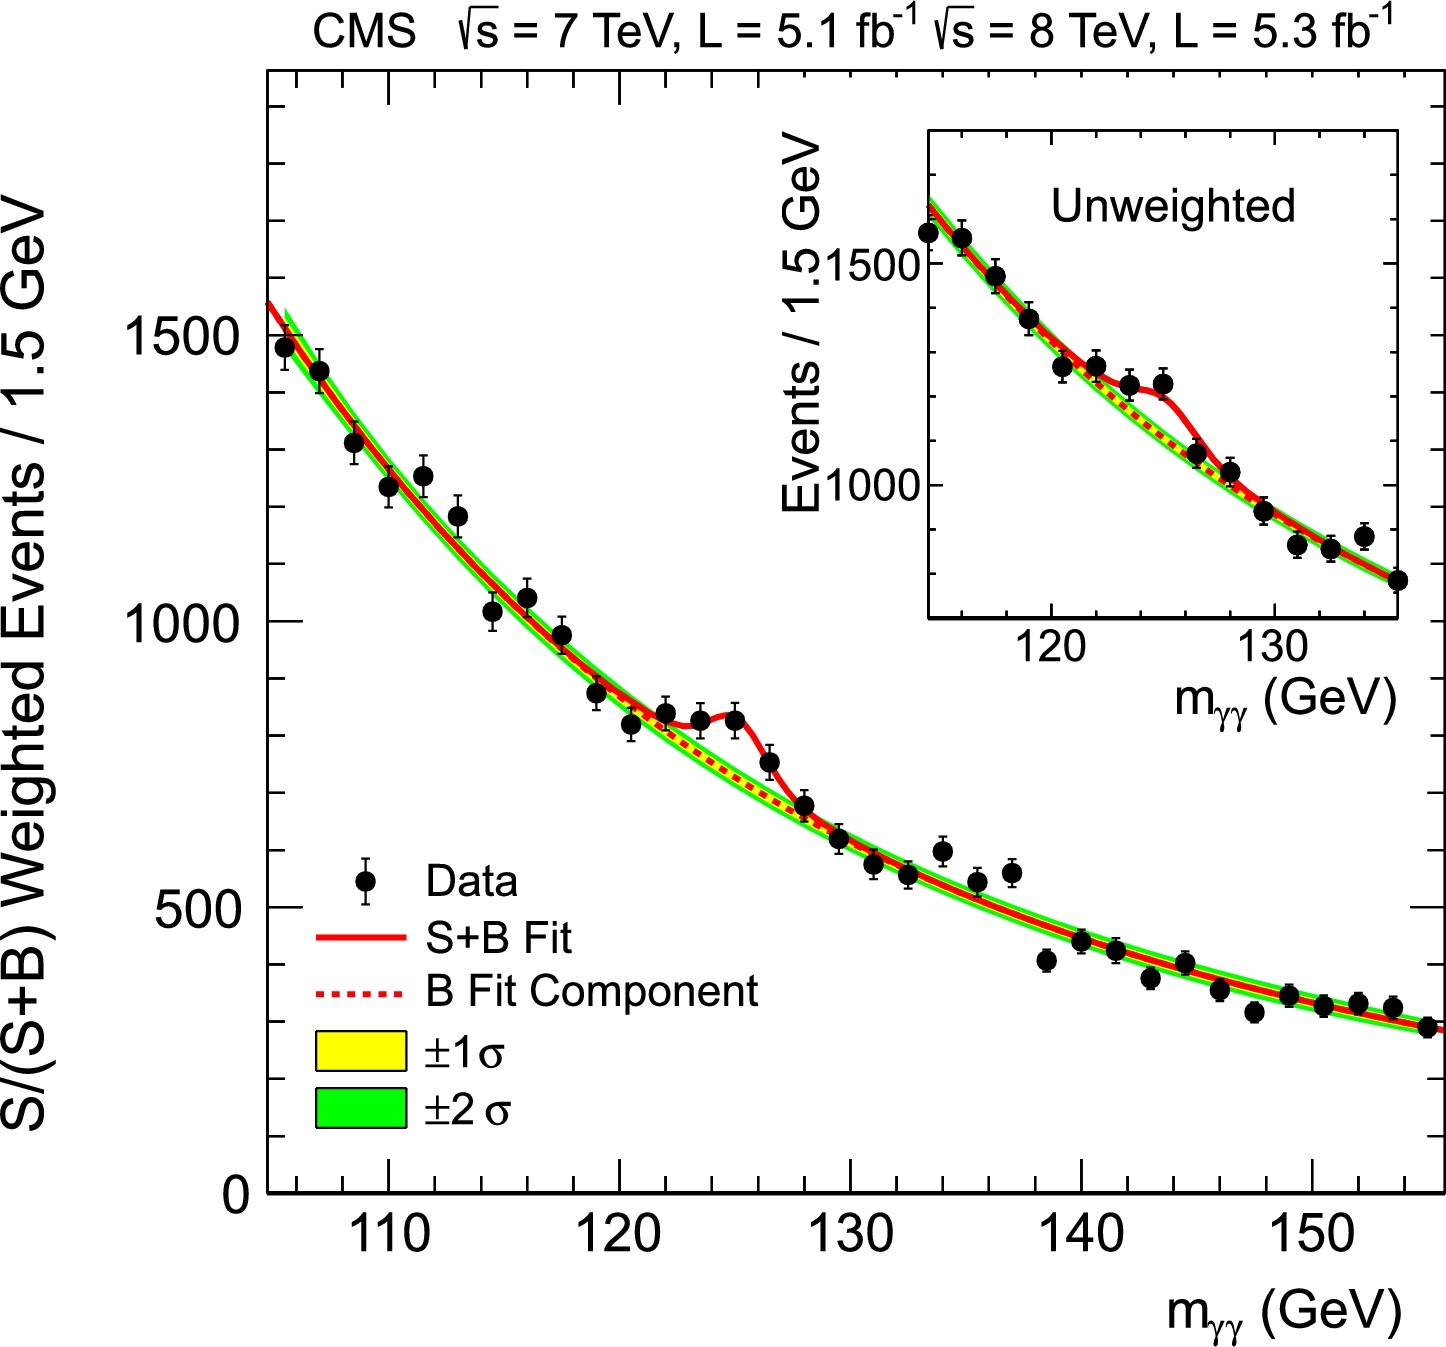
\includegraphics[width=0.45\textwidth]{Figures/c1/higgs_2.jpeg}
\caption{Left, ``distribution of the four-lepton invariant mass for the $ZZ\rightarrow 4\ell$ analysis. The points represent the data, the filled histograms represent the background, and the open histogram shows the signal expectation for a Higgs boson of mass , added to the background expectation''~\cite{201230}. Right, ``the diphoton invariant mass distribution with each event weighted by the S/(S + B) value of its category. The lines represent the fitted background and signal, and the colored bands represent the $\pm$1 and $\pm$2 standard deviation uncertainties in the background estimate''~\cite{201230}.}
\label{fig:higgmass}
\end{figure}

It was observed for the first time by ATLAS~\cite{20121} and CMS~\cite{201230} experiments in 2012.
About CMS results, they were searches for the Higgs boson in pp collisions at 7\TeV and 8\TeV corresponding to an integrated luminosity of 5.1\fbinv and 5.3\fbinv respectively. The search was carried out in five decay modes, but the most significant excess above the expected background was observed in the two decay modes that provide the best mass resolution: $h^{0} \rightarrow ZZ$ and $h^{0} \rightarrow \gamma \gamma$. The final signal and background yields are shown in Figure~\ref{fig:higgmass}. An excess of events with local significance of 5.0$\sigma$ was found 125\GeV.\\
From the observed decay modes, it was inferred that the new particle, $h^{0}$ is a boson with spin that is not equal to one since it decays into two photons. Finally, $h^0$ has no electric charge, and it has weak isospin $T_3=-1/2$ and hypercharge $Y=1$.

Once the mass problem of the \PW and \PZ bosons is fixed, it is necessary to address the problem of the generation of the mass terms for the SM fermions. Introducing Yukawa interactions between fermions and the scalar field into the SM Lagrangian, the mass terms for SM fermions are fixed:
\begin{equation}
\label{eq:yukawa}
 \mathcal{L}_{\text{Yukawa}} \;\; = \;\; -\lambda^{ij}_dq^{-i}_L\phi d^j_R \;-\; \lambda^{ij}_uq^{-i}_L\tilde{\phi} u^j_R \;-\; \lambda^{ij}_{\ell}\overline{\ell}^{-i}_L\phi e^j_R \;+\; \text{hermitian conjugate}
\end{equation}
where $\tilde{\phi}= i\sigma\phi^*$, $q_L$ is a LH quark doublet, $u_R$ and $d_R$ are RH up and down quark singlets, $\ell_L$ is the LH doublet of leptons while $e_R$ is the RH lepton singlet. $\lambda^{ij}_u$, $\lambda^{ij}_d$ and $\lambda^{ij}_\ell$ are the up-quark, down-quark and lepton Yukawa coupling strengths ($i,j$ being the generation indices). \\
In Eq.~\ref{eq:yukawa}, the Yukawa Lagrangian, it is clear the absence of the mass term for the neutrinos; this remark is going to be crucial when the neutrino flavor oscillation observations will be presented.

To conclude, while the boson mass terms are determined by a gauge principle, the fermionic couplings with the Higgs field are not. Consequently, the corresponding Yukawa coupling constants (or the fermionic masses) are free parameters of the theory in contrast with the bosons masses which 
 are established by the couplings of the gauge interactions and the VEV of the Higgs field.



\section{Beyond the Standard Model}\label{sec:bsm}
The SM describes exceptionally well nearly all the processes that have been observed in particle physics, and its predictions do agree with an outstanding level of accuracy with the results from numerous precision measurements. Even though the theory has not shown any decisive evidence of where it can fail or where the formulation can be inaccurate, we know by now the SM does not cover the full picture and there are several indications that other fundamental physics remains to be unmasked.

In this section a few of the open questions in physics are very briefly listed and described trying to show why new physics beyond the SM is to be expected. Furthermore, some simplified explanations of such possible theories or extensions are provided. They will be discussed either the scenarios with additional particles and symmetries or the introduction of a more general theory for very high energies while considering the SM as an effective theory at current or lower energy scales.\\
Taking into account the context of this work, the focus will be heavily steered towards the introduction of RH heavy neutrinos as Beyond the SM theory and solution.



\subsection{Open questions of the Standard Model}\label{sec:questions}
\subsubsection{Gravity}
The Standard Model does not contain a description of gravitational interactions therefore being incomplete and failing to incorporate the general relativity theory in the SM theory itself. Proposals to describe gravity as a quantum field theory have included a possible spin-2 boson, called graviton, as mediator of the gravitational force; however, no experimental evidence have been found up to now. 

\subsubsection{Dark matter and dark energy}

It is well known today from several unquestionable cosmological observations that only roughly 5$\%$ of all the energy content of the universe consists of the baryonic matter as defined and included in the SM, then so-called \emph{ordinary matter}. In the standard $\Lambda$CDM model of cosmology, on top of the $\approx 5\%$ of ordinary matter, about 27\% is made up of another kind of matter that appears to be not directly visible (it does not interact with the electromagnetic field) and thus is so-called \emph{Dark Matter} (DM). The residual 68\% is called \emph{Dark Energy}. Hence DM is 85\% of the total mass and up to know we can fully describe and predict only 5\% of the universe. The values are obtained from observation of the CMB (cosmic microwave background) by the Planck satellite and published in this exhaustive review~\cite{2020Plank}.

There are several cosmological observational evidence for dark matter. We can cite the calculations of the velocity dispersion and the rotation curves of galaxies, the gravitational lensing measurements and the distribution of the cosmic microwave background; additionally there are the astronomical observations of the universe's current structure and the formation and evolution of structures as galaxies and nebulas.\\
\begin{figure}[h]
\centering
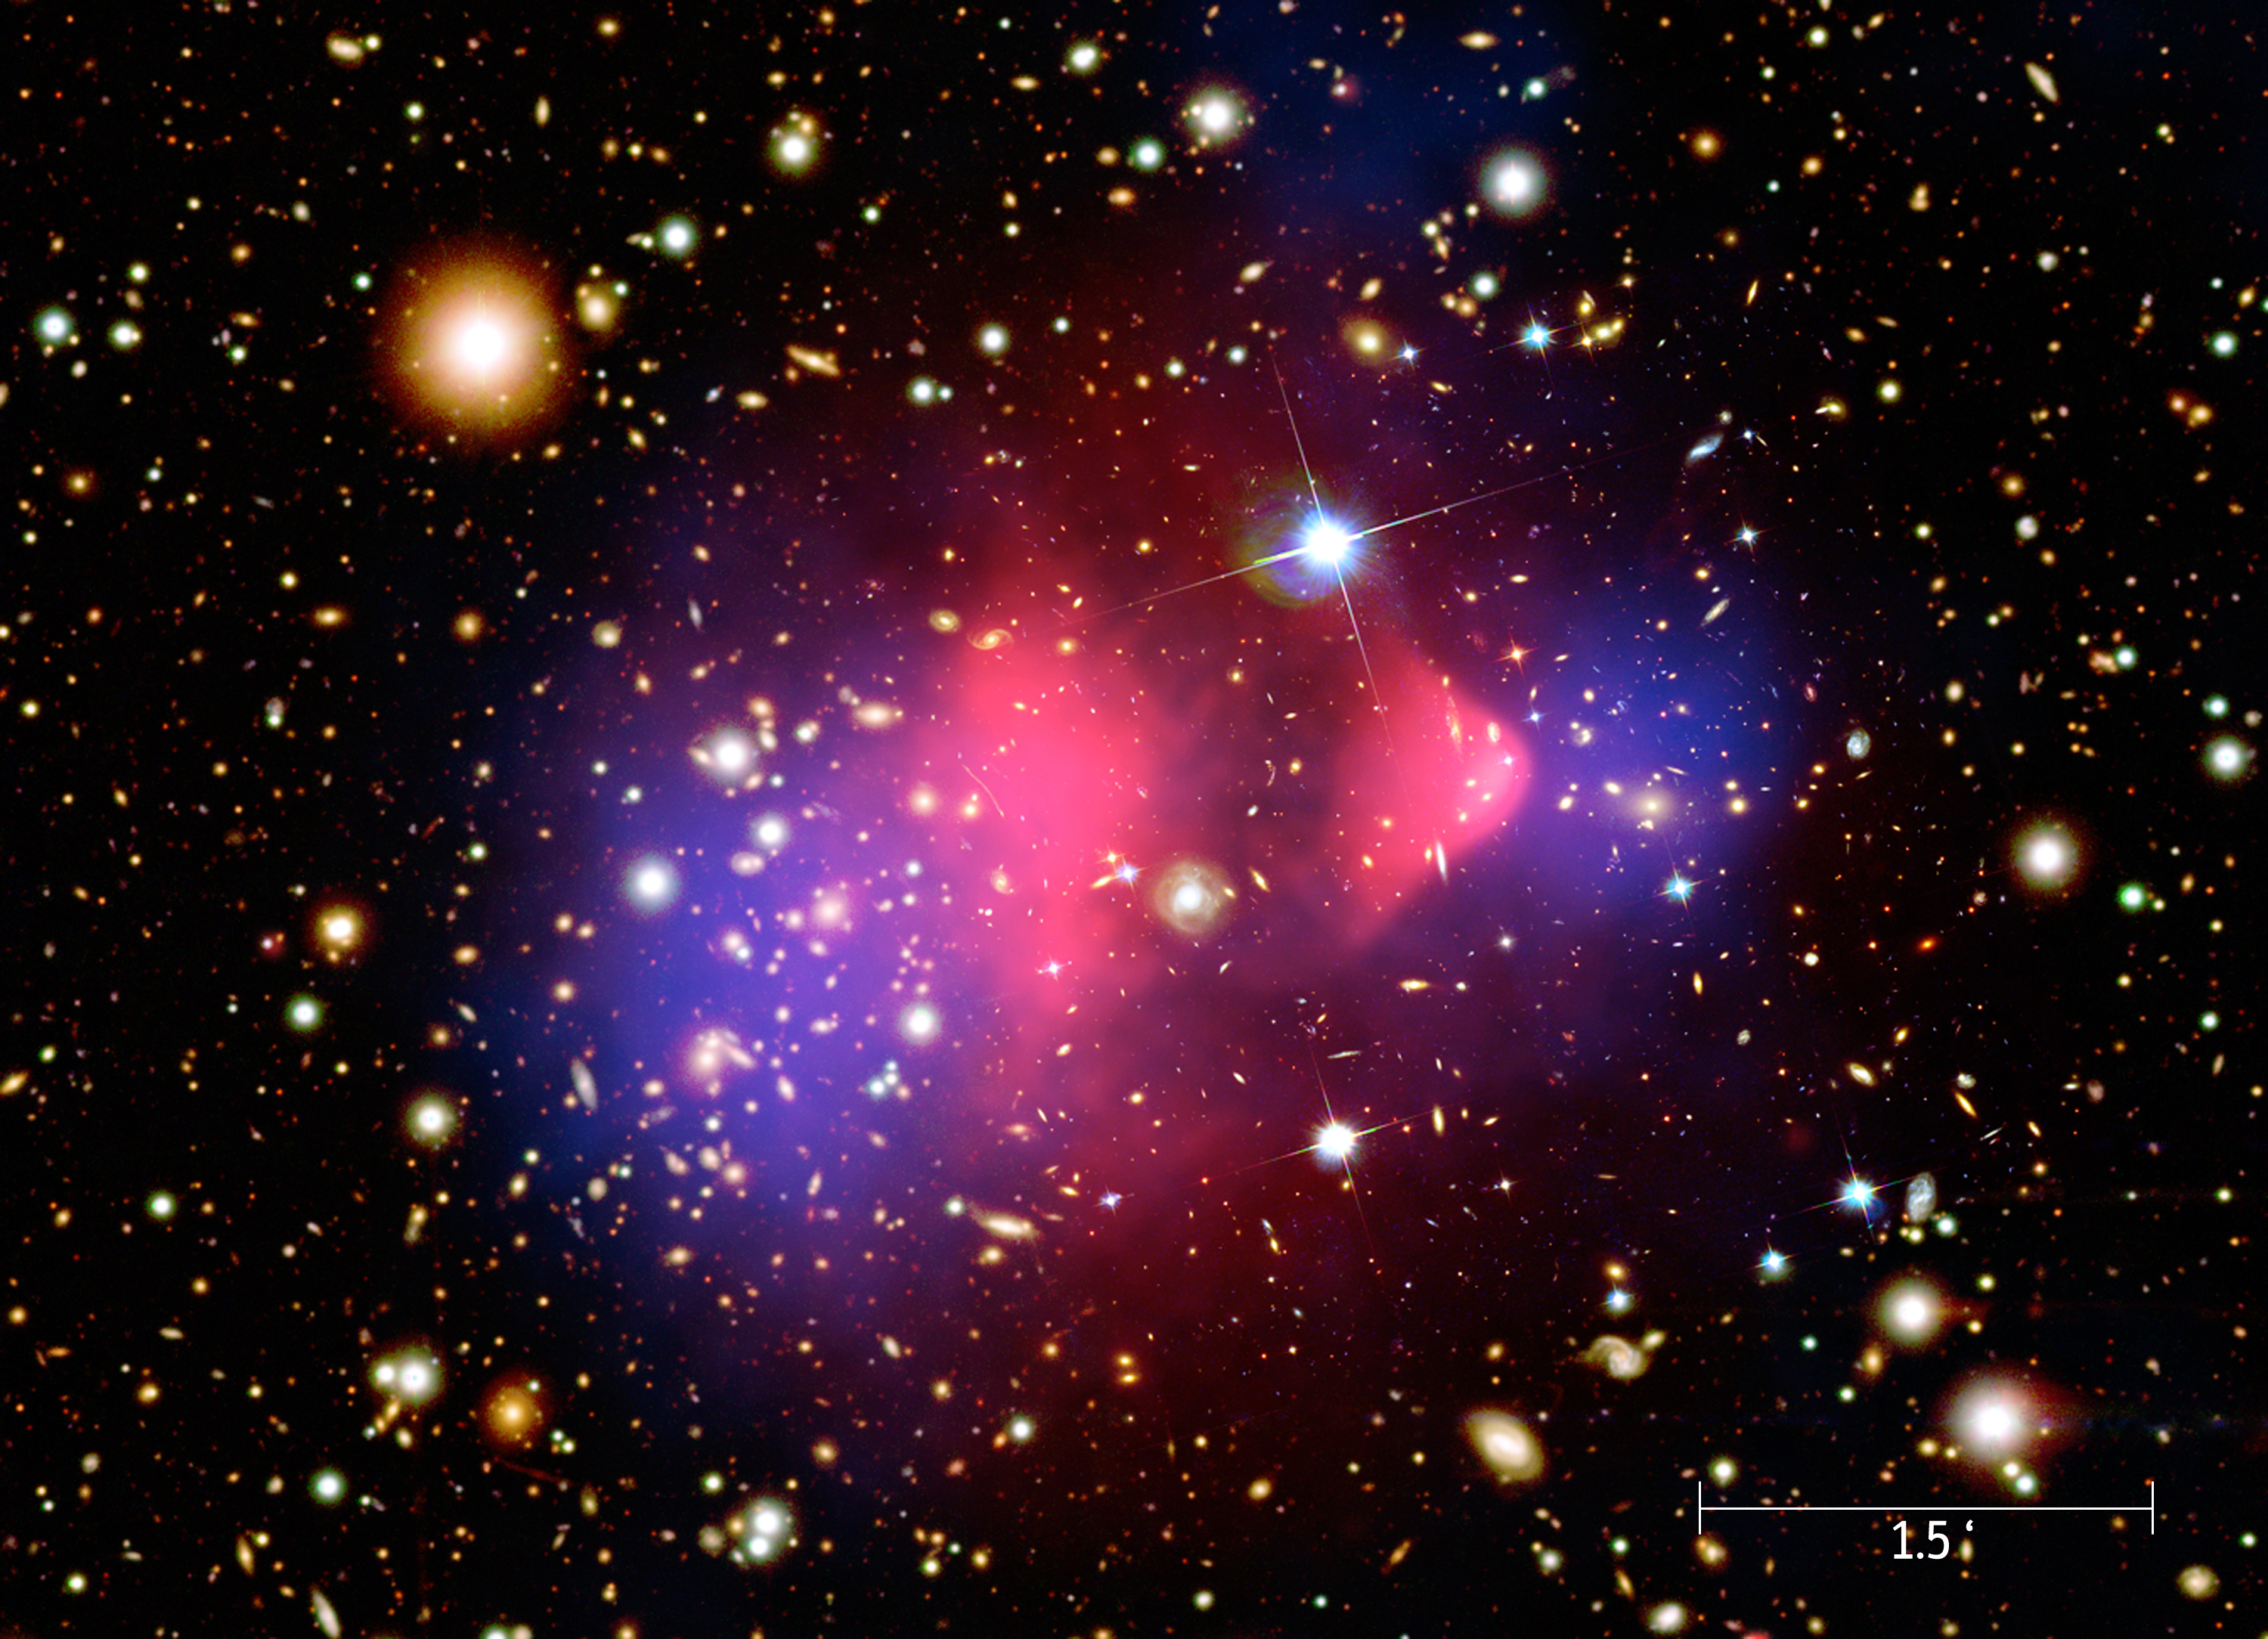
\includegraphics[width=0.65\textwidth]{Figures/c1/bullet.jpg}
\caption{X-ray image (pink) superimposed over a visible light imagine (galaxies) with the matter distribution (DM plus ordinary matter) calculated from gravitational lensing (blue)~\cite{webpage_bullet}}
\label{fig:bullet}
\end{figure}
An interesting and very clear example is the one coming from the observation of the \emph{Bullet Cluster} (1E 0657-56)~\cite{Clowe_2004} (see Fig.~\ref{fig:bullet}) which is a transparent proof of DM. The \emph{Bullet Cluster} indicates a smaller sub-cluster (on the right in Fig.~\ref{fig:bullet}) moving away from a larger one in a bigger structure consisting of two colliding clusters of galaxies. Comparing the information obtained through X-rays measurements, which quantify the hot gas of baryonic matter, with the total amount of matter (DM plus ordinary matter) detected indirectly by the gravitational lensing of background objects, the Bullet Cluster provides 
one of the best evidence to date for the existence of dark matter. With a statistical significance of 8$\sigma$ it was addressed that ``spatial offset of the center of the total mass from the center of the baryonic mass peaks cannot be explained with an alteration of the gravitational force law alone, and thus proves that the majority of the matter in the system is unseen''~\cite{Clowe_2006}.

All cosmological evidence of DM relies on its gravitational effects, which is the only type of interaction that, up to now, DM is expected to have with ordinary matter.\\
Since it is still unknown which is the nature of DM, dark matter searches are one of the hottest and most fascinating  topics in both particle physics and theoretical physics. Several experiments have tried to detect DM through either direct detection or indirect detection and via collider experiments where the DM candidate could be produced in the collision of leptonic or hadronic beams. For clear reviews of DM searches at the CMS Experiment see~\cite{LOWETTE2016503,Bhawna_Gomber}.

Many candidates for DM have been sifted, some being part of more structured theories like Supersymmetry or others being completely new exotic particles. To give a simple list of possible solutions, candidates for non-baryonic dark matter could be particles like axions, weakly interacting massive particles (WIMPs),  gravitationally-interacting massive particles (GIMPs), supersymmetric particles and sterile neutrinos. The latter are very interesting in the scenario of this thesis work too, providing an excellent aspirant as DM~\cite{DREWES2017250,Cline_2020}. Sterile neutrinos (or neutral leptons) are defined to interact only via gravity and do not couple with any gauge fields of the SM, hence the name \emph{sterile} to distinguish them from the \emph{active} neutrinos of the SM. In the following references a few interesting models with sterile neutrinos as DM candidate are listed~\cite{Davidson_2008,PhysRevLett.72.17,PhysRevD.64.023501,KUSENKO20091,DOLGOV2002339}.


\subsubsection{Baryon asymmetry and CP violation}
The baryon asymmetry problem is also known as the matter-antimatter asymmetry problem and outlines the imbalance between the baryonic matter and the anti-baryonic matter in the observable universe.\\
 At the Big Bang instant, it is believed the same amount of matter and antimatter was produced, but the clear disproportion we observe today and in the early universe suggests that some physical laws must have operated differently for matter and antimatter. As proposed in 1967 by Andrei Sakharov~\cite{Sakharov:1967dj}, this matter-antimatter asymmetry can only be justified if the theory allows for a violation of charge-conjugation symmetry and of parity symmetry\footnote{Parity transformation is the inversion of the sign of one of the spatial coordinates; P-symmetry refers to equations and processes with are invariant under mirror inversions. All the interactions of elementary particles but weak interaction are symmetric under parity.}; these simultaneous violations are so-called CP violation. \\
The first observation of indirect CP violation was provided in 1964 by James Cronin and by Val Fitch with the ``the Fitch-Cronin Experiment''~\cite{PhysRevLett.13.138} where clear evidence was found of CP violation in neutral kaons decays.\\
For a direct CP violation proof, we needed to wait till 1999 for the results from KTeV experiment~\cite{Alavi_Harati_1999} at Fermilab and the observation from the NA48 experiment~\cite{Fanti_1999} at CERN. The most recent updates come from the LHCb experiment which has announced the discovery of CP violation in neutral D meson decay~\cite{PhysRevLett.122.211803}.

The sterile neutrinos, previously mentioned, are seen as possible candidates to address the matter-antimatter asymmetry problem thanks to their different behaviors under CP transformation with respect to Dirac neutrinos. In the following references~\cite{Gandhi_2015,Klop_2015,Palazzo_2020}  there are a few examples of experimental results interpretations with the sterile neutrinos in the context of CP violation theories.

\subsubsection{Neutrino masses}
In Eq.~\ref{eq:yukawa}, the Yukawa Lagrangian, it is clear the absence of the mass term for the neutrinos. As mentioned and explained in Sec~\ref{sec:ewk} (Eq.~\ref{eq:LR2}), it is in principle possible to add the mass term as a RH component in the Lagrangian. Nevertheless, up to this day, the RH neutrinos have not been found and it is expected to be very difficult to observe them knowing that the RH fermions do transform as singlets under the entire SM gauge group and consequently they are sterile. It was then accepted for a long time that the neutrinos would be massless particles in nature.

The whole understanding of neutrinos within the boundaries of the SM was shaken and weakened in 1968 with the results from the Brookhaven National Laboratory obtained with the Brookhaven solar neutrino detector~\cite{PhysRevLett.20.1205}.
It was observed that the number of electron neutrinos coming from the sun was significantly lower with respect to the expected value using solar-model calculations of the neutrino flux from decay of ${}^{8}B$\footnote{For the experiment at the Brookhaven National Laboratory, the calculations of the flux of solar neutrino coming from boron-8 decay were used: ${}^{8}B\rightarrow {}^{8}Be + e^{+} + \nu_e$. For a simple scheme and explanation see webpage~\cite{webpage_boron}.} inside the sun. This was the first hint of the so-called \emph{solar neutrino problem}.\\
The explanation for this deficiency and for the other observed ``neutrino anomalies'' during those years was found to be the existence of neutrino flavor oscillations, theoretically predicted in 1957 by Bruno Pontecorvo~\cite{osti_4343073}. \\
The first crucial evidence for these speculations arrived in 1998 with the results from Super-Kamiokande Observatory~\cite{Fukuda_1998}. The data showed an angularly dependent deficit of muon neutrinos, $\nu_{\mu}$ which is not consistent with the expectations based on the calculation of the atmospheric neutrino flux. The difference in angular distribution between neutrinos coming from above the detector and the one coming from below (going through the earth) suggested a higher survival probability for $\nu_{\mu}$ traveling a shorter distance.\\
The first direct observation of the oscillation of the electron neutrino to other flavors was only in 2001~\cite{Ahmad_2001} at the Sudbury Neutrino Observatory in Canada. The experiment was designed to detect solar neutrinos from the decay of ${}^{8}B$ via the charged current (CC) reaction on ${}^{2}H$ and by elastic scattering (ES) of electrons; the first reaction (CC) was sensitive only to $\nu_e$, while the ES reaction also to  $\nu_{\mu}$ and $\nu_{\tau}$. Starting from the assumption that the fusion processes in the sun produce only electron neutrinos, a flux of $\nu_{e}$ equal to the one calculated from ${}^{8}B$  decays was expected. The total flux of electron neutrino was instead found to be much lower than the predictions (as for~\cite{PhysRevLett.20.1205}) but the total rate, $\nu_{e} + \nu_{\mu} + \nu_{\tau}$ was surprisingly in line with the number of neutrinos expected to arrive from the sun. This was the first direct evidence of the neutrino flavor oscillation, \ie neutrinos change flavor when traveling long distances. The phenomenon in which a neutrino can be created with a specific lepton number and then, after being propagated through space, can be measured to have a different lepton number, is called neutrino oscillation and it can happen only if the neutrinos have a non-zero mass. Then, the main question would be how the neutrino masses arise.

One of the most promising explanations is the addition of the Majorana mass term in Eq.~\ref{eq:yukawa}. This theory, which is the main topic of this thesis, is going to be extensively explored in Chapter~\ref{Chapter3}.

\clearpage
\section{Summary}\label{sec:summaryC1}
In this chapter it was presented the Standard Model of particle physics.
The elementary particles, 
their properties and the fundamental forces with their force carriers were introduced. 
In the Standard Model, the elementary particles are grouped into two main categories on the basis of the statistic they obey: fermions and bosons. The fermions, specifically quarks, charged leptons and neutral leptons form what we name matter. The fermions interact by exchanging bosons which are force carriers and each of them is associated with a fundamental force: the photon ($\gamma$) is the mediator of the electromagnetic force, the $\PW^{\pm}$ and \PZ are mediators of the weak force and the gluons are mediators for the strong force.
To complete the picture, it was introduced the Brout–Englert–Higgs (BEH) mechanism which refers to the generation of masses for the three weak massive gauge bosons (\PW, \PZ) through electroweak symmetry breaking.\\
A short historical walk-through of the Standard Model discoveries and milestones is presented as well as a description of the mathematical framework of the Standard Model of particle physics, the gauge Quantum Field Theory.

Then we selected a few challenges that particle
physics encounters: the baryon asymmetry, new physics in the neutrino field and
the inquiry for Dark Matter. All the three items are subjects of the two searches presented in the last two chapters of this work. In this thesis the focus will be steered towards the introduction, the explanation and then the quest of the Heavy Neutral Leptons. \\
First the CMS experiment will be introduced in Chapters~\ref{Chapter2} and~\ref{Chapter2_5}, then the Heavy Neutral Leptons model will be explained in Chapter~\ref{Chapter3} trying to show the reason behind the huge enthusiasm about this topic which has lead in the past $\sim10$ years to the creation of a very active community and to the publication of an impressive numbers of papers and the proposal of a considerable number of new experiments. Considering that, finally the two searches for Heavy Neutral Leptons at CMS are presented in Chapters~\ref{Chapter5} and~\ref{Chapter6} at which the author has firsthand participated during her PhD.


